\chapter{Arquitectura de programación}
El término arquitectura del conjunto de instrucciones (instruction set architecture) (ISA) se refiere al conjunto de instrucciones visibles al programador. Funciona como la frontera entre el software y el hardware.

\begin{center}
 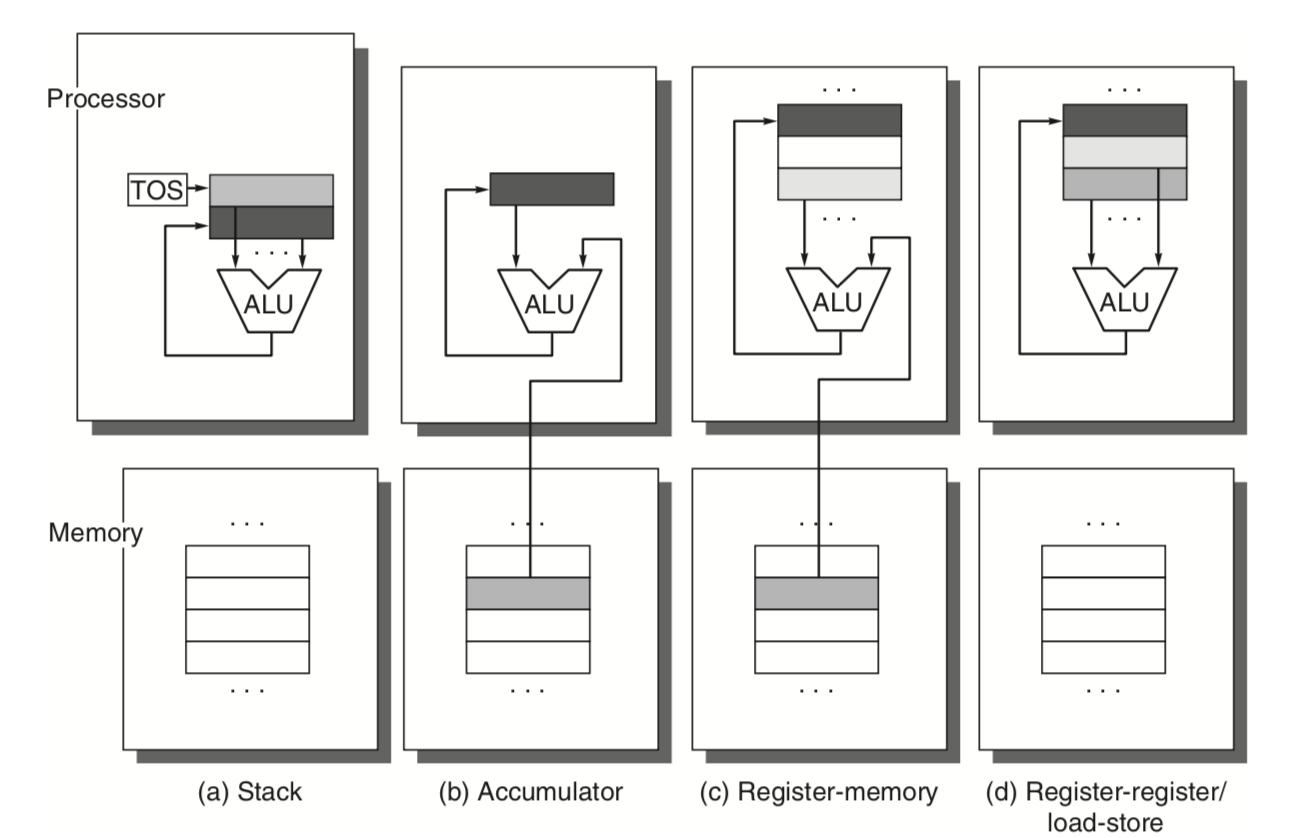
\includegraphics[scale=.6,keepaspectratio=true]{gfx/ISA.png}
\end{center}


\section{Modelo de pila}
Los operandos en una arquitectura de stack están implícitamente en el tope del stack y el hardware debe evaluar la expresión en un solo orden y cargar un operando múltiples veces.


\section{Modelo de acumulador}
En una arquitectura de acumulador un operando está implícito en el acumulador.


\section{Modelo de registros de propósito general}
En la arquitectura de registros de propósito general se tienen únicamente operandos explícitos, ya sea que estén ubicados en registros o en memoria.

Los operandos explícitos podrían ser accedidos directamente de memoria o necesitar ser cargados de memoria a un registro temporal dependiendo de la arquitectura y de la instrucción específica.


\section{Modelo de carga y almacenamiento}
En este tipo de arquitectura, la memoria solo puede ser accedida a través de instrucciones de carga y almacenamiento (load/store). 

\subsection{Conjunto de instrucciones RISC}
Las arquitecturas RISC se caracterizan por tener ciertas propiedades que simplifican su implementación.

\begin{itemize}
\item Todas las operaciones de datos aplican a datos en registros y típicamente modifican todo el registro (32 o 64 bits por registro).
\item Las únicas operaciones que afectan a la memoria son de carga y almacenamiento (load y stores) que mueven datos de la memoria a un registro o viceversa. Estas operaciones pueden mover datos menores que la capacidad de un registro (por ejemplo 16 bits).
\item El número de formatos de instrucciones son pocos con todas las instrucciones del mismo tamaño.
\end{itemize}

Como otras arquitecturas RISC, el conjunto de instrucciones de MIPS tiene 32 registros, aunque el registro 0 siempre tiene el valor 0. 

Hay tres tipos de instrucciones:

\begin{enumerate}
\item Instrucciones ALU. Estas instrucciones toman dos registros o bien un registro y un inmediato de signo extendido, realiza la operación y almacena el resultado en otro registro.

\item Instrucciones Load / Store. Estas instrucciones toman un registro base, y un inmediato como offset. La suma resultante del contenido del registro y el offset da la dirección efectiva y es usada para direccionar la memoria. En el caso de un store, el segundo registro opera como fuente del dato que se almacena en memoria.

\item Branches  y  jumps. Branches son transferencias condicionales del flujo de control. La forma de especificar la condición del branch, MIPS compara entre un par de registros o entre un registro y cero.

El destino del branch se obtiene sumando un offset con extensión de signo (16 bits) al valor actual del PC.
\end{enumerate}

\begin{center}
 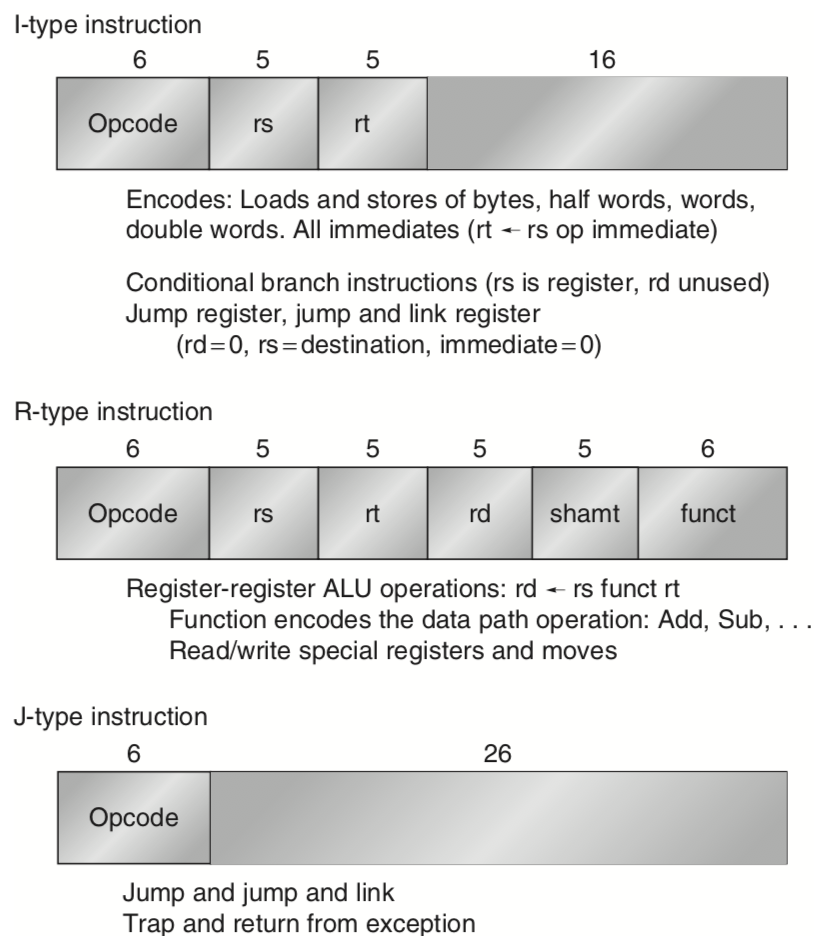
\includegraphics[scale=.65,keepaspectratio=true]{gfx/tipos_instruccion.png}[h!]
\end{center}

\subsection{Direccionamiento de memoria}
Independientemente de la arquitectura, si es load-store o una que permita a cualquier operación tener una referencia a memoria, se debe definir como son interpretadas las direcciones de memoria y como se especifican.

Todo el conjunto de instrucciones es direccionado por bytes y se provee acceso por bytes (8 bits), mitad de palabra (half words) (16 bits), por palabra (words) (32 bits).

Hay dos convenciones para ordenar los bytes en un objeto. \textbf{Little Endian} coloca el byte cuya dirección "x . . . x000” en la posición menos significativa. Los bytes entonces son numerados:

\begin{center}
 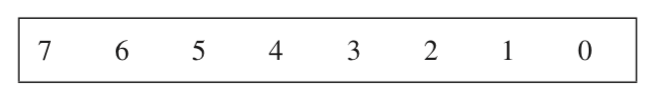
\includegraphics[scale=.7,keepaspectratio=true]{gfx/little_endian.png}[h!]
\end{center}


El orden \textbf{Big Endian} coloca el byte cuya dirección es “x . . . x000”  en la posición más significativa. Los bytes entonces son numerados:

\begin{center}
 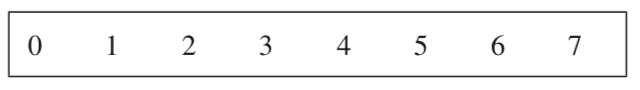
\includegraphics[scale=.7,keepaspectratio=true]{gfx/big_endian.png}[h!]
\end{center}

El orden de los bytes es un problema cuando se intercambia datos entre computadoras con diferentes ordenamientos. Por ejemplo cuando se comparan strings, en Little Endian aparece “SDRAWKCAB” (backwards) en los registros.


\subsection{Registros} 
MIPS64 tiene 32 registros de propósito general de 64-bit (GPRs) llamados R0, R1,..., R31. 
Además tiene 32 registros de punto flotante, F0, F1,..., F31, que pueden almacenar 32 valores de simple precisión o 32 valores de doble precisión (64-bit). Cuando se almacena un valor de precisión simple, la otra mitad del registro no se utiliza. 

El valor del registro R0 es siempre cero.


\subsection{Tipo de datos}
Los tipo de datos son bytes de 8-bit, half words de 16-bit, words de 32-bit y double words de 64-bit para enteros y datos de 32-bit de precisión simple y 64-bit de doble precisión para punto flotante.


\subsection{Operaciones}
Las operaciones en MIPS64 trabajan en enteros de 64-bit o punto flotante de 32 o 64-bit. Bytes, half words, y words son cargados en los registros de propósito general con ceros o con el bit de signo para llenar los 64 bits.


\subsection{Modos de direccionamiento}
Los únicos modos de direccionamiento son inmediato o por desplazamiento, ambos con campos de 16-bit. Por registro indirecto se logra al ubicar 0 en los 16-bit del campo de desplazamiento y direccionamiento absoluto se logra al usar el registro cero como registro base.

